\chapter{Datasets} \label{sec:appendix_datasets}

\begin{table}
\centering
\tabcolsep=0.1cm
\begin{tabular}{llrrr}
\toprule
\textbf{dataset} & \textbf{alias} & \textbf{dim} & \textbf{anom} & \textbf{normal}   \\\midrule
ANNthyroid & ann  & 21 & 534 & 6665 \\
Arrhythmia & arr  & 275 & 206 & 245 \\
HAR & har & 561 & 1944 & 8355  \\
HTRU2 & htr & 8 & 1638 & 16257  \\
KDD99 (10\%) & kdd & 118 & 396742 & 97276  \\
Mammography & mam & 6 & 260 & 10921  \\
Seismic & sei  & 24 & 170 & 2412  \\
Spambase & spm & 57 & 1812 & 2786  \\
\midrule
Abalone & aba & 10 & 50 & 2151  \\
Blood Transfusion & blt & 4 & 16 & 382  \\
Breast Cancer Wisconsin & bcw  & 30 & 206 & 356 \\
Breast Tissue & bts & 9 & 22 & 65 \\
Cardiotocography & crd & 27 & 228 & 1830  \\
Ecoli & eco & 7 & 108 & 205  \\
Glass & gls & 10 & 94 & 112  \\
Haberman & hab & 3 & 14 & 225  \\
Ionosphere & ion & 33 & 122 & 225  \\
Iris & irs & 4 & 46 & 100  \\
Isolet & iso & 617 & 3300 & 4496  \\
Letter Recognition & ltr & 617 & 3600 & 4196  \\
Libras & lbr & 90 & 142 & 215  \\
Magic Telescope & mgc & 10 & 3882 & 12331  \\
Miniboone & mnb & 50 & 23922 & 93565  \\
Multiple Features & mlt & 649 & 800 & 1200  \\
PageBlocks & pgb & 10 & 384 & 4911  \\
Parkinsons & prk & 22 & 44 & 146  \\
Pendigits & pen & 16 & 5384 & 5537  \\
Pima Indians & pim & 8 & 176 & 500  \\
Sonar & snr & 60 & 96 & 110  \\
Spect Heart & sph & 44 & 52 & 211  \\
Statlog Satimage & sat & 36 & 2630 & 3592  \\
Statlog Segment & seg & 18 & 938 & 1320  \\
Statlog Shuttle & sht & 8 & 28 & 57767  \\
Statlog Vehicle & vhc & 18 & 132 & 627  \\
Synthetic Control Chart & scc & 60 & 200 & 400  \\
Wall Following Robot & wrb & 24 & 2220 & 2921  \\
Waveform-1 & wf1 & 21 & 1482 & 3302  \\
Waveform-2 & wf2 & 21 & 1472 & 3302  \\
Wine & wne & 13 & 70 & 106  \\
Yeast & yst & 8 & 390 & 751   \\\bottomrule
\end{tabular}
\vspace*{0.15cm}
\caption{Basic statistics of the tabular dataset designed for anomaly detection  (above split) and multi-class datasets  (bellow split).}
\label{tab:tabular_datasets}
\end{table}

\begin{table}
    \centering
    \tabcolsep=0.1cm
    \begin{tabular}{lllrr}
    \toprule
    \textbf{dataset} & \textbf{alias} & \textbf{dim} & \textbf{anom} & \textbf{normal} \\
    \midrule
    MNIST-C & mnistc & 28x28x1 & 70000 & 70000 \\
    MVTec-AD - wood & wood & 1024x1024x3 & 60 & 266 \\
    MVTec-AD - grid & grid & 1024x1024x3 & 57 & 285 \\
    MVTec-AD - transistor & transistor & 1024x1024x3 & 40 & 273 \\
    \midrule
    CIFAR10 & cifar10 & 32x32x3 & 54000 & 6000  \\
    FashionMNIST & fmnist & 28x28x1 & 63000 & 7000   \\
    MNIST & mnist & 28x28x1 & 63686 & 6312  \\
    SVHN2 & svhn2 & 32x32x3 & 80327 & 18960  \\\bottomrule
    \end{tabular}
    \vspace*{0.15cm}
    \caption{Basic statistics of image datasets designed for anomaly detection (above split) and multi-class datasets (below split).}
    \label{tab:image_datasets}
\end{table}


\begin{figure}
    \centering
    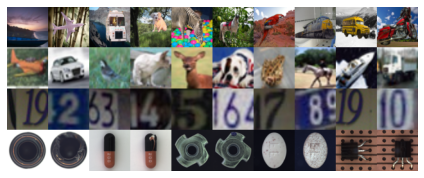
\includegraphics[width=\textwidth]{data/chapter_sgvaegan/fig5_all_grid.png}
    \caption{Examples of the datasets used in the experiments. Datasets from the top row to bottom: COCOPlaces, CIFAR10, SVHN2, and MVTec-AD. MVTec-AD examples of normal and anomalous samples from the \textit{bottle, capsule, metal nut, pill}, and \textit{transistor} classes are shown.}
    \label{fig:all_grid}
\end{figure}

\begin{description}
    \item[\textbf{Wildlife MNIST}]~\cite{sauer2021counterfactual} is an artificial dataset based on standard MNIST~\cite{lecun2010mnist}. For each MNIST digit, a background and foreground texture is sampled from a texture dataset described in~\cite{cimpoi2014describing} to create a colored version. Two versions of this dataset were created - \textit{mixed} and \textit{non-mixed}. In the mixed version, the background and foreground for each digit are sampled randomly from 10 background and foreground texture classes to create a very diverse set of images. In the non-mixed version, the background and foreground class is kept the same for all basic MNIST digits from the same class, resulting in a less diverse dataset. For examples of the non-mixed version, see the top row of Fig.~\ref{fig:wmnist_grid}. Each version contains 60000 samples of 32x32 pixel RGB images with three factors of variation.
    
    \item[\textbf{COCOPlaces}] is a dataset created similarly to Wildlife MNIST. 10 classes of objects from the COCO dataset~\cite{lin2014microsoft} were combined with 10 background classes from the Places dataset~\cite{zhou2017places}. Again, mixed and non-mixed variants were created. Because the object shape and texture cannot be separated in this case, it represents a problem with two factors of variation that is slightly more realistic than the previous one. Furthermore, it is much harder, as the object shapes are very distinct, sometimes the foreground object is only partially visible and the background itself may sometimes contain some other objects as well. A total of 5000 64x64 pixel RGB images were generated for each variant. For sample images of all classes, see~Fig.~\ref{fig:all_grid}.
    % the object classes are 'boat', 'airplane', 'truck','dog','zebra','horse','bird','train','bus','motorcycle'
    % the background classes are 'beach', 'bamboo_forest','canyon','broadleaf forest','ball_pit','orchard','rock_arch','shower','ski_slope','wheat_field'

    \item[\textbf{SVHN2}] is a well-known benchmark dataset~\cite{netzer2011reading} containing images of house numbers. In this cropped version of the dataset, the target digit is centered in the middle of the picture. However, there may be partial digits adjacent to it, which makes the problem harder. Furthermore, there are no available annotations for the background/foreground factor and in this paper, it is included mainly as a benchmark for comparison to other baseline methods. There are 10 classes for a total of 99288 32x32 pixel RGB images. The distribution of classes is uneven and ranges from 6 to 19 thousand samples. 
    
    \item[\textbf{CIFAR10}] is another classical dataset of images of 10 classes of different objects or animals often used for validation of anomaly detectors~\cite{ruff2018deep, ruff2019deep, chalapathy2018anomaly}. For an overview of the dataset see~\cite{krizhevsky2009learning}. There is a total of 60000 32x32 pixel RGB images.

    \item[\textbf{MVTec-AD}] is an industrial dataset~\cite{bergmann2019mvtec} that captures several different problems of identifying faulty or damaged objects. We have considered only the problems where there is a distinct object in the foreground, such as \textit{bottle} or \textit{metal nut}. The individual problems are smaller --- on average about 200 normal and 100 anomalous samples. The images used in our experiments are downscaled to 128x128 pixels.
    
\end{description}


The CIFAR10~\cite{krizhevsky2009learning}, SVHN22~\cite{netzer2011reading} and MVTec-AD~\cite{bergmann2019mvtec} are publicly available datasets. 